% Options for packages loaded elsewhere
\PassOptionsToPackage{unicode}{hyperref}
\PassOptionsToPackage{hyphens}{url}
%
\documentclass[
]{article}
\usepackage{lmodern}
\usepackage{amssymb,amsmath}
\usepackage{ifxetex,ifluatex}
\ifnum 0\ifxetex 1\fi\ifluatex 1\fi=0 % if pdftex
  \usepackage[T1]{fontenc}
  \usepackage[utf8]{inputenc}
  \usepackage{textcomp} % provide euro and other symbols
\else % if luatex or xetex
  \usepackage{unicode-math}
  \defaultfontfeatures{Scale=MatchLowercase}
  \defaultfontfeatures[\rmfamily]{Ligatures=TeX,Scale=1}
\fi
% Use upquote if available, for straight quotes in verbatim environments
\IfFileExists{upquote.sty}{\usepackage{upquote}}{}
\IfFileExists{microtype.sty}{% use microtype if available
  \usepackage[]{microtype}
  \UseMicrotypeSet[protrusion]{basicmath} % disable protrusion for tt fonts
}{}
\makeatletter
\@ifundefined{KOMAClassName}{% if non-KOMA class
  \IfFileExists{parskip.sty}{%
    \usepackage{parskip}
  }{% else
    \setlength{\parindent}{0pt}
    \setlength{\parskip}{6pt plus 2pt minus 1pt}}
}{% if KOMA class
  \KOMAoptions{parskip=half}}
\makeatother
\usepackage{xcolor}
\IfFileExists{xurl.sty}{\usepackage{xurl}}{} % add URL line breaks if available
\IfFileExists{bookmark.sty}{\usepackage{bookmark}}{\usepackage{hyperref}}
\hypersetup{
  pdftitle={Sustainability of Brazilian forest concessions},
  hidelinks,
  pdfcreator={LaTeX via pandoc}}
\urlstyle{same} % disable monospaced font for URLs
\usepackage[margin=1in]{geometry}
\usepackage{longtable,booktabs}
% Correct order of tables after \paragraph or \subparagraph
\usepackage{etoolbox}
\makeatletter
\patchcmd\longtable{\par}{\if@noskipsec\mbox{}\fi\par}{}{}
\makeatother
% Allow footnotes in longtable head/foot
\IfFileExists{footnotehyper.sty}{\usepackage{footnotehyper}}{\usepackage{footnote}}
\makesavenoteenv{longtable}
\usepackage{graphicx,grffile}
\makeatletter
\def\maxwidth{\ifdim\Gin@nat@width>\linewidth\linewidth\else\Gin@nat@width\fi}
\def\maxheight{\ifdim\Gin@nat@height>\textheight\textheight\else\Gin@nat@height\fi}
\makeatother
% Scale images if necessary, so that they will not overflow the page
% margins by default, and it is still possible to overwrite the defaults
% using explicit options in \includegraphics[width, height, ...]{}
\setkeys{Gin}{width=\maxwidth,height=\maxheight,keepaspectratio}
% Set default figure placement to htbp
\makeatletter
\def\fps@figure{htbp}
\makeatother
\setlength{\emergencystretch}{3em} % prevent overfull lines
\providecommand{\tightlist}{%
  \setlength{\itemsep}{0pt}\setlength{\parskip}{0pt}}
\setcounter{secnumdepth}{5}
\usepackage{booktabs}
\usepackage{longtable}
\usepackage{array}
\usepackage{multirow}
\usepackage{wrapfig}
\usepackage{float}
\usepackage{colortbl}
\usepackage{pdflscape}
\usepackage{tabu}
\usepackage{threeparttable}
\usepackage{threeparttablex}
\usepackage[normalem]{ulem}
\usepackage{makecell}
\usepackage{xcolor}

\title{Sustainability of Brazilian forest concessions}
\author{}
\date{\vspace{-2.5em}}

\begin{document}
\maketitle

{
\setcounter{tocdepth}{2}
\tableofcontents
}
\hypertarget{introduction}{%
\section{Introduction}\label{introduction}}

Legal logging in the tropics is typically governed by simple rules that set a minimum cutting diameter and a minimum cutting cycle of 25-35 years (Putz et al. 2008). Timber harvests in diverse forests are selective because few species are marketable and few trees meet the size and bole quality requirements. In the Amazon, selective logging regulations typically set a rotation cycle of 20 to 35 years with a logging intensity varying from 15 to 30 m\(^3\) of harvested timber per ha. Such rules, promulgated by governments since the middle of last century, are generally based on an assumed post-logging rate of commercial timber volume increments of about 1 m\(^3\).ha\(^{-1}\).year\(^{-1}\) (0.86 m\(^3\).ha\(^{-1}\).year\(^{-1}\) in Brazilian Amazon). These rules are set to accommodate processing technologies and market demands, rather than the biology and conservation of the harvested species (Sist and Ferreira 2007). Unfortunately for the goal of sustainability, research reports over the past decades demonstrated that volume recovery rates fall short of this expectation by 50\% (reviewed by Putz et al. 2012). A recent simulation of post-logging timber volume recovery rates in the Amazon Basin showed that even with cutting cycles of 65 years and logging intensities of only 20 m\(^3\).ha\(^{-1}\), logged forests recover only 70\% of their pre-logging timber stocks (Piponiot et al. 2019). Other researchers showed that current harvest regimes can only be sustained over multiple cycles if high-value slow-growing hardwoods are replaced by fast-growing species with low density wood of little market value (Alder and Silva 2000; Keller et al. 2004; Phillips et al. 2004; Gardingen, Valle, and Thompson 2006; Sist and Ferreira 2007; Schulze, Grogan, and Vidal 2008). Here we use a timber recovery model (Piponiot et al. 2019) to estimate the timber volumes that could be produced by all the logging concessions in the Brazilian Amazon with different cutting cycle lengths, logging intensities, and lengths of the list of commercial species.

Despite low rates of post-harvest timber stock recovery, selective logging is still widespread and economically important land use in the tropics in general and Amazon Basin in particular. In that region, forest degradation due to illegal logging is widespread (Brancalion et al. 2018; Finer et al. 2014; Potapov et al. 2017) and, in the Brazilian Amazon, affects now bigger areas than deforestation ({\textbf{???}}). This makes difficult to assess the region's current potential for timber production. What is clear, in contrast, is that without control of illegal logging and improved practices where logging is legal, timber yields from logged forests will decline dramatically (Putz et al. 2012; Piponiot et al. 2019), decreasing the likelihood of their meeting the demand for timber.

In 2006, the Brazilian Forest Service (SFB) was created to establish a very ambitious system of long-term logging concessions (Brazil 2006). The goals are to provide a legal framework for sustainable timber production in Amazonian forests while reducing illegal logging. Forest concessions in the Brazilian Amazon currently cover only 1.6 million ha (SFB 2019a), but the maximum potential area is estimated up to 60 million ha (Bomfim et al. 2016). The current timber production rate from established forest concessions is 221,000 m\(^3\) per year, which is only 2\% of the timber extracted from the region (SFB 2019a). Given that these concessions are to be managed with a 50 cm minimum cutting diameter (with the exception of \emph{Swientenia macrophylla}: 60 cm) and a 25-35 year cutting cycle coupled with rising demand for wood products, the assessment of the expected timber production from these forests over the long term is warranted.

In this paper we assess the timber yield sustainability of different logging intensities and harvest cycle durations from forest concessions in the Brazilian Amazon. We assess whether the potential annual timber production is adequate to meet the estimated present timber demand of 11 Mm\(^3\).yr\(^{-1}\) (Vidal et al. 2020; SFB 2019a).

\hypertarget{methods}{%
\section{Methods}\label{methods}}

\hypertarget{study-areas---brazilian-concessions}{%
\subsection{Study areas - Brazilian concessions}\label{study-areas---brazilian-concessions}}

Our study focuses on forest concessions in the Brazilian Amazon (Fig. \ref{fig:map-brazil-concess}). These concessions are located in public forests and currently cover 1.6 Mha, of which 1.05 Mha are managed by the SFB, and 0.6 Mha are managed by state-level agencies (SFB 2019a). We defined the area of all potential concessions as the area of all public forests that (i) are in the Brazilian Amazon biome, (ii) are designated for sustainable use, and (iii) are not community forests - although community forest management is legal and currently cover around 260.000 ha ({\textbf{???}}), indigenous territories or military areas (as defined in SFB (2019a), p.~112; Fig. \ref{fig:map-brazil-concess}{]}. Based on this definition, the potential concession area in the Brazilian Amazon cover an estimated of 35 Mha. This area is lower than the 60 Mha estimated by Bomfim et al. (2016); xxx explanation.

\begin{figure}
\centering
\includegraphics{br_concessions_files/figure-latex/map-brazil-concess-1.pdf}
\caption{\label{fig:map-brazil-concess}Forest concessions in the Brazilian Amazon. Current federal concessions are in red; potential concessions (public forests designated for sustainable use) are in blue {[}retrieved from Brazilian Forest Service and IDEFLOR websites (SFB 2020, 2019b; IDEFLOR-BIO n.d.){]}.}
\end{figure}

\hypertarget{the-vdde-model}{%
\subsection{The VDDE model}\label{the-vdde-model}}

In this study we used the volume dynamics with differential equations model (VDDE) (Piponiot et al. 2018). The VDDE model calculates the volume of all live trees \(\geq\) 50 cm diameter at breast height (DBH), the standard minimum cutting size in the Brazilian Amazon. The portion of this volume composed of commercial species is referred to as the commercial volume.

The input variables set for each simulation are logging intensity, logging cycle length, and the initial proportion of the volume that is commercial (\(\omega_0\)). Low values of \(\omega_0\) represent highly selective logging where only the most valuable species are harvested whereas high values mean that most species are logged. Other parameters of the VDDE model are spatially defined at a 1\(^\circ\) resolution. The model was calibrated for the Amazon Basin with a Bayesian framework with data from 3500 ha of forest plots, among which 845 ha are from 15 sites monitored for as long as 30 years after selective logging (Sist et al. 2015; Piponiot et al. 2019). Predictions of commercial volume recovery rates thereby vary with location.

Each logging cycle includes the harvest itself as a function of logging intensity and forest characteristics and the post-logging volume recovery phase, which varies with logging cycle length and forest characteristics. Logging lowers both the total volume and the proportion of commercial volume, but both then increase during the recovery phase, although the proportion of commercial volume takes longer to recover because it relies solely on the recruitment of trees \textless{} 50 cm DBH (Piponiot et al. 2019). These two steps are sequentially repeated to simulate 1000 years of logging.

The results are then multiplied by the area of current or potential concessions in each 1\(^\circ\) pixel, and by a factor \(\pi \sim \mathcal{Beta}(8.2, 5.9)\) between 0 and 1, with a mean value of 58\%. This factor \(\pi\), which was calibrated with data from logging concessions in French Guiana, reflects the ratio between logged areas and the initially allocated areas, mostly because of slope restrictions and riparian reserves, but also heavy forest degradation because of illegal logging and other disturbances (Verissimo et al. 2006; Piponiot et al. 2019).

Uncertainties are propagated throughout the model by drawing all parameter values from their calibrated distribution (from Piponiot et al. 2019), and simulating logging cycles with these parameter values. This process is repeated 100 times and summary statistics (medians and 95\% credibility intervals) are calculated at each time step.

\hypertarget{testing-scenarios}{%
\subsection{Testing scenarios}\label{testing-scenarios}}

We tested 27 different scenarios by using combinations of the following inputs: (i) initial proportion of commercial volume: 20\% (highly selective), 50\% (intermediate) or 90\% (non-selective); (ii) logging intensity: 10 m3.ha-1 (low), 20 m\(^3\).ha\(^{-1}\) (intermediate) or 30 m\(^3\).ha\(^{-1}\) (high); (iii) cutting cycle length: 20 years (short), 35 years (intermediate) or 60 years (long). These scenarios are then applied to the current area of concessions and to the area of all potential concessions (see ``Study areas'').

For each scenario we simulated 1000 years of logging cycles, and determined the duration of maintained timber production, i.e.~the time before timber stocks become insufficient to maintain a constant timber production as illustrated in Fig. \ref{fig:illust-sust-log}. This maintained production is different from sustained timber production which theoretically shows a constant timber yield and stock over time (Fig. \ref{fig:illust-sust-log}).

\begin{figure}
\centering
\includegraphics{br_concessions_files/figure-latex/illust-sust-log-1.pdf}
\caption{\label{fig:illust-sust-log}Illustration of the duration of maintained and sustained timber production. The x-axis represents years after the first selective harvest, and the y-axis represents commercial volumes as simulated by the model with a logging intensity of 10 m\(^3\).ha\(^{-1}\) and a logging cycle of 60 years. At each harvest, commercial volumes decrease (blue segments). If logging cycles are not long enough to allow recovery, the commercial volume decreases until it is not sufficient to maintain a constant production (10, 20 or 30 m\(^3\).ha\(^{-1}\), red segments). The time taken to reach this limit is the duration of the maintained production. In the sustained timber production, both timber yield and stocks remain constant.}
\end{figure}

\hypertarget{results}{%
\section{Results}\label{results}}

\begin{figure}
\centering
\includegraphics{br_concessions_files/figure-latex/tsust-vs-prodi-1.pdf}
\caption{\label{fig:tsust-vs-prodi}Tradeoff between timber production and sustainability. The x-axis is the annual timber production under each scenario, and in all areas considered in the scenario (left panels: current concessions; right panels: potential concessions). The y-axis is the duration of constant production in each scenario, in years. The points are the median value over all simulations for each scenario; the vertical and horizontal error bars are the 95\% credibility intervals. Colors represent logging rules (3 logging intensities x 3 logging cycle lengths) and the 3 values of initial proportion of commercial volume (\(\omega_0\)) are represented by different panels, in increasing order from top to bottom. The target production of timber is 11 Mm\(^3\).yr\(^{-1}\), corresponding to the current timber production in Brazilian Amazonian forests. Only a few scenarios in the right panels (all potential concessions) are above this target, and all of them have a median duration of constant production lower than 200 years.}
\end{figure}

\textbackslash begin\{table\}

\textbackslash caption\{\label{tab:sust-production}Sustainability of all 27 scenarios, characterized by the duration of constant timber production (yrs, last 2 columns). The first 3 columns correspond to the input variables: the proportion of commercial volume (\%); logging intensity (m\(^3\).ha\(^{-1}\)); logging cycle length (yr). The last column is the duration of constant timber production in potential concession areas, as the median value of all iterations, followed by the 95\% credibility interval (between parentheses).\}
\centering

\begin{tabular}[t]{l|l|l|l}
\hline
Comm. volume & Log. intensity & Log. cycle & Duration of maintained prod.\\
\hline
 &  & 20 yr & 20 yr (20 - 60)\\
\cline{3-4}
 &  & 35 yr & 35 yr (35 - 105)\\
\cline{3-4}
 & \multirow{-3}{*}{\raggedright\arraybackslash 10 m\$\textasciicircum{}3\$.ha\$\textasciicircum{}\{-1\}\$} & 60 yr & 60 yr (60 - 180)\\
\cline{2-4}
 &  & 20 yr & 20 yr (20 - 20)\\
\cline{3-4}
\cellcolor{lightgrey}{} & \cellcolor{lightgrey}{} & \cellcolor{lightgrey}{35 yr} & \cellcolor{lightgrey}{35 yr (35 - 35)}\\
\cline{3-4}
 & \multirow{-3}{*}{\raggedright\arraybackslash 20 m\$\textasciicircum{}3\$.ha\$\textasciicircum{}\{-1\}\$} & 60 yr & 60 yr (60 - 60)\\
\cline{2-4}
 &  & 20 yr & 20 yr (20 - 20)\\
\cline{3-4}
 &  & 35 yr & 35 yr (35 - 35)\\
\cline{3-4}
\multirow{-9}{*}{\raggedright\arraybackslash 20\%} & \multirow{-3}{*}{\raggedright\arraybackslash 30 m\$\textasciicircum{}3\$.ha\$\textasciicircum{}\{-1\}\$} & 60 yr & 60 yr (60 - 60)\\
\cline{1-4}
 &  & 20 yr & 80 yr (20 - 160)\\
\cline{3-4}
 &  & 35 yr & 210 yr (35 - 385)\\
\cline{3-4}
\textbf{} & \textbf{\multirow{-3}{*}{\raggedright\arraybackslash 10 m\$\textasciicircum{}3\$.ha\$\textasciicircum{}\{-1\}\$}} & \textbf{60 yr} & \textbf{540 yr (60 - >1000)}\\
\cline{2-4}
 &  & 20 yr & 40 yr (20 - 60)\\
\cline{3-4}
 &  & 35 yr & 70 yr (35 - 140)\\
\cline{3-4}
 & \multirow{-3}{*}{\raggedright\arraybackslash 20 m\$\textasciicircum{}3\$.ha\$\textasciicircum{}\{-1\}\$} & 60 yr & 120 yr (60 - 300)\\
\cline{2-4}
 &  & 20 yr & 20 yr (20 - 40)\\
\cline{3-4}
 &  & 35 yr & 35 yr (35 - 70)\\
\cline{3-4}
\multirow{-9}{*}{\raggedright\arraybackslash 50\%} & \multirow{-3}{*}{\raggedright\arraybackslash 30 m\$\textasciicircum{}3\$.ha\$\textasciicircum{}\{-1\}\$} & 60 yr & 60 yr (60 - 120)\\
\cline{1-4}
 &  & 20 yr & 220 yr (20 - 520)\\
\cline{3-4}
\textbf{} & \textbf{} & \textbf{35 yr} & \textbf{>1000 yr (70 - >1000)}\\
\cline{3-4}
\textbf{} & \textbf{\multirow{-3}{*}{\raggedright\arraybackslash 10 m\$\textasciicircum{}3\$.ha\$\textasciicircum{}\{-1\}\$}} & \textbf{60 yr} & \textbf{>1000 yr (960 - >1000)}\\
\cline{2-4}
 &  & 20 yr & 80 yr (20 - 140)\\
\cline{3-4}
 &  & 35 yr & 175 yr (35 - 350)\\
\cline{3-4}
\textbf{} & \textbf{\multirow{-3}{*}{\raggedright\arraybackslash 20 m\$\textasciicircum{}3\$.ha\$\textasciicircum{}\{-1\}\$}} & \textbf{60 yr} & \textbf{780 yr (60 - >1000)}\\
\cline{2-4}
 &  & 20 yr & 40 yr (20 - 80)\\
\cline{3-4}
 &  & 35 yr & 70 yr (35 - 175)\\
\cline{3-4}
\multirow{-9}{*}{\raggedright\arraybackslash 90\%} & \multirow{-3}{*}{\raggedright\arraybackslash 30 m\$\textasciicircum{}3\$.ha\$\textasciicircum{}\{-1\}\$} & 60 yr & 240 yr (60 - 480)\\
\hline
\end{tabular}

\textbackslash end\{table\}

\begin{figure}
\centering
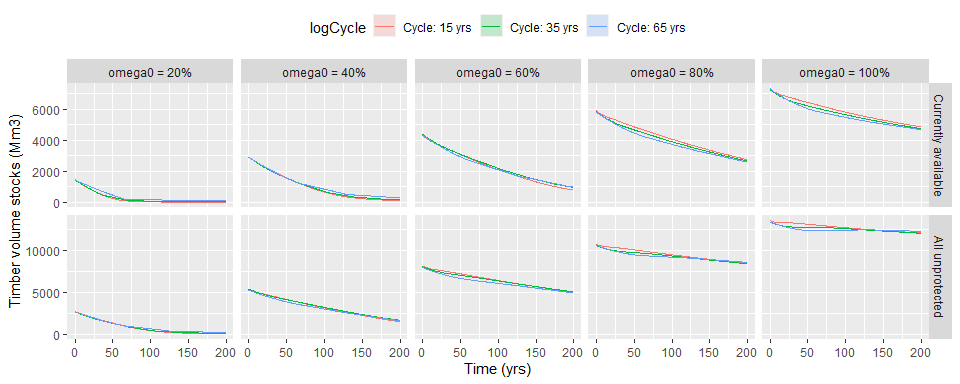
\includegraphics{br_concessions_files/figure-latex/timber-stocks-1.pdf}
\caption{\label{fig:timber-stocks}Commercial volume stocks in all potential concession areas for the 4 scenarios with a duration of maintained production \textgreater{} 500 years. The x-axis is the time after the first logging event (in years); the y-axis is the commercial volume stocks in all potential concession areas, in Mm\(^3\). The colors represent the 4 scenarios, with the thick lines corresponding to the median and the shaded areas to the 95\% credibility interval over all iterations.}
\end{figure}

None of the scenarios with an initial commercial volume proportion of 20\% are sustainable after the first logging cycle (Fig. \ref{fig:tsust-vs-prodi}; Table \ref{tab:sust-production}). The present logging practices in the Brazilian Amazon usually correspond to a proportion of commercial species of \textless{} 20\%, a mean logging intensity of 15-20 m\(^3\).ha\(^{-1}\) and a rotation cycle of 35 years. Under such rules, the timber production can be maintained only for a single cutting cycle (35 years, grey line in Table \ref{tab:sust-production}). Scenarios with higher proportion of commercial timber show longer duration of maintained production: 70 yr (35 - 140) and 175 yr (35 - 350) when the proportion of commercial species is respectively 50\% and 90\%.

Only 4 out of all 27 scenarios (bold lines in Table \ref{tab:sust-production}) have median durations of maintained production over 500 years, and only one is close to a sustained timber production \emph{sensu stricto} (10 m\(^3\).ha\(^{-1}\) every 60 years with a 90\% initial proportion of commercial timber species, Fig. \ref{fig:timber-stocks}). Three of these scenarios have an initial proportion of commercial volume of 90\%, and two correspond to low intensity logging (10 m\(^3\).ha\(^{-1}\)) with a cutting cycle of 60 years (Table \ref{tab:sust-production}).

The current timber production from the Brazilian Amazon is around 11 Mm\(^3\) per year (Vidal et al. 2020; SFB 2019a). Current concessions cannot come close to satisfying this demand for even one cycle under any scenario (Fig. \ref{fig:tsust-vs-prodi}). The maximum annual production from the current concession areas is 1.43 Mm\(^3\).yr\(^{-1}\), which can only be reached under the most intensive scenarios: 30 m\(^3\).ha\(^{-1}\) of timber extracted every 20 years, with an initial proportion of commercial timber \(\geq\) 50\% (Fig. \ref{fig:tsust-vs-prodi}). Under such conditions, the maximum duration of maintained production is 40 yr (20 - 80) (Fig. \ref{fig:tsust-vs-prodi}). Under the present harvesting practices of 20 m\(^3\).ha\(^{-1}\) every 35 years with only 20\% of the volume of trees \(\geq\) 50 cm DBH of commercial species, the annual production from the first harvest is only 473,000 m\(^3\) and the production will not be maintained after the first cutting cycle (35 years). Finally, with the current concession area, the longest maintained timber production (780 years) reaches 317.000 m\(^3\) under an extraction rate of 20 m\(^3\).ha\(^{-1}\) every 60 years with a 90\% proportion of commercial species (Fig. \ref{fig:tsust-vs-prodi}).

When considering all potential concession areas (35 Mha), the annual production of 11 Mm\(^3\).yr\(^{-1}\) could be maintained, at best, for 175 yr (35-350) if 90\% of the volume is commercial, logging intensity is 20 m\(^3\).ha\(^{-1}\) and cutting cycles are 35 years (Fig. \ref{fig:tsust-vs-prodi}; Table \ref{tab:sust-production}). The two others scenarios that yield close to 11 Mm\(^3\) with a sustained duration of 250 years (Fig. \ref{fig:tsust-vs-prodi}) use logging intensities of 10 and 30 m3.ha-1 and logging cycles of 20 and 60 years, respectively. Under current rules (20 m\(^3\).ha\(^{-1}\) every 35 years and 20\% proportion of commercial timber) the total annual production is 10Mm\(^3\).yr\(^{-1}\) but the sustained timber production will be only for 35 years, which means that this production can be sustained only for two cutting cycles (Figure 3).

\hypertarget{discussion}{%
\section{Discussion}\label{discussion}}

\begin{itemize}
\item
  methods: optimistic hypotheses -\textgreater{} to be considered when interpreting results -\textgreater{} Camille
\item
  According to the results of our simulations, several challenges must be faced to reach sustained timber production within the concession systems in the Brazilian Amazon. First, the proportion of commercial species must increase considerably at least to 50\% but ideally to 90\%. Second, the logging intensity must be reduced to 10 m\(^3\).ha\(^{-1}\) and the rotation cycle to 60 years. Third, the area of current concessions is obviously insufficient to reach an annual production of 11 Mm\(^3\) and it is urgent to increase drastically concession area to its maximum potential of 35 Mha. However, the potential concession area of 35 Mha show strong limitation to ensure a annual sustainable production of 11 Mm\(^3\) on a long term basis as our simulations suggest that this production can be sustained for at best 170 years with a 90\% proportion of commercial species.
\item
  This study confirms that the present regulation fixing a rotation cycle of 35 years cannot ensure a long term sustainable timber production. Although previous studies already demonstrated the need to change the present extraction rates (Sist and Ferreira 2007, Putz et al.~2008, other refs) our paper is the first one suggesting and assessing different options of logging practices. The main challenge to move towards more sustainable practices is undoubtedly to increase the proportion of commercial species from presently 20 \% to 90\%. This must involve drastic changes at all level but particularly in the industrial and market sectors. At present, the wood transformation industry is still technically very poorly developed and very rudimentary (refs?). Less than 30\% of the logs entering the saw mill is transformed, the remaining 70\% are wasted and burned. However, the lack of wood transformation technology is certainly linked to the lack of market demand on diversified wood products in the region. To be developed (Jack ? Edson ?)
\item
  increasing the area of concessions: current trends, challenges and opportunities
\item
  initial proportion of commercial species: what effect could harvesting 90\% of all trees \textgreater{} 50 cm DBH could have on the profitability of selective logging?
\item
  initiating a forest transition -\textgreater{} new ways of producing timber: plantations, active restoration, silviculture
\item
  what effects could silviculture have on sustainability? -\textgreater{} needs to be investigated (introduce next paper)
\end{itemize}

\hypertarget{references}{%
\section*{References}\label{references}}
\addcontentsline{toc}{section}{References}

\hypertarget{refs}{}
\leavevmode\hypertarget{ref-Alder2000}{}%
Alder, D, and Jnm Silva. 2000. ``An empirical cohort model for management of TerraFirme forests in the Brazilian Amazon.'' \emph{Forest Ecology and Management} 130: 141--57. \url{http://linkinghub.elsevier.com/retrieve/pii/S0378112799001966}.

\leavevmode\hypertarget{ref-Bomfim2016}{}%
Bomfim, Sergio Luiz do, Alexandre Louis de Almeida D'Avignon, Álvaro Nogueira de Souza, Paulo José Prudente de Fontes, and Maísa Santos Joaquim. 2016. ``O potencial da concessão de florestas públicas para o desenvolvimento socioeconômico e geração de emprego na Amazônia Legal.'' \emph{Revista Do Serviço Público} 67 (4): 649--70. \url{https://doi.org/10.21874/rsp.v67i4.759}.

\leavevmode\hypertarget{ref-Brancalion2018}{}%
Brancalion, Pedro H. S., Danilo R. A. de Almeida, Edson Vidal, Paulo G. Molin, Vanessa E. Sontag, Saulo E. X. F. Souza, and Mark D. Schulze. 2018. ``Fake legal logging in the Brazilian Amazon.'' \emph{Science Advances} 4 (8): eaat1192. \url{https://doi.org/10.1126/sciadv.aat1192}.

\leavevmode\hypertarget{ref-Brazil2006}{}%
Brazil. 2006. ``Lei n 11.284/2006. Dispõe sobre a lei gestão de florestas públicas para a produção sustentável; institui, na estrutura do Ministério do Meio Ambiente, o Serviço Florestal Brasileiro - SFB; cria o Fundo Nacional de Desenvolvimento Flores- tal - FNDF; e dá.'' \url{http://www.planalto.gov.br/ccivil\%7B/_\%7D03/\%7B/_\%7DAto2004-2006/2006/Lei/L11284.htm}.

\leavevmode\hypertarget{ref-Finer2014}{}%
Finer, Matt, Clinton N. Jenkins, Melissa A Blue Sky, and Justin Pine. 2014. ``Logging Concessions Enable Illegal Logging Crisis in the Peruvian Amazon.'' \emph{Scientific Reports} 4 (4719): 1--6. \url{https://doi.org/10.1038/srep04719}.

\leavevmode\hypertarget{ref-VanGardingen2006}{}%
Gardingen, Paul R. van, Denis Valle, and Ian Thompson. 2006. ``Evaluation of yield regulation options for primary forest in Tapaj??s National Forest, Brazil.'' \emph{Forest Ecology and Management} 231 (1-3): 184--95. \url{https://doi.org/10.1016/j.foreco.2006.05.047}.

\leavevmode\hypertarget{ref-IDEFLOR2020}{}%
IDEFLOR-BIO. n.d. ``Contratos de Concessão Florestal.'' Accessed February 17, 2021. \url{https://ideflorbio.pa.gov.br/contratos-de-concessao-florestal/}.

\leavevmode\hypertarget{ref-Keller2004}{}%
Keller, Michael, Michael Palace, Gregory P. Asner, Rodrigo Pereira, and Jose Natalino M. Silva. 2004. ``Coarse woody debris in undisturbed and logged forests in the eastern Brazilian Amazon.'' \emph{Global Change Biology} 10 (5): 784--95. \url{https://doi.org/10.1111/j.1529-8817.2003.00770.x}.

\leavevmode\hypertarget{ref-Phillips2004}{}%
Phillips, P. D, C. P de Azevedo, B. Degen, I. S Thompson, J. N. M Silva, and P. R van Gardingen. 2004. ``An individual-based spatially explicit simulation model for strategic forest management planning in the eastern Amazon.'' \emph{Ecological Modelling} 173 (4): 335--54. \url{https://doi.org/10.1016/j.ecolmodel.2003.09.023}.

\leavevmode\hypertarget{ref-Piponiot2018}{}%
Piponiot, Camille, Géraldine Derroire, Laurent Descroix, Lucas Mazzei, Ervan Rutishauser, Plinio Sist, and Bruno Hérault. 2018. ``Assessing timber volume recovery after disturbance in tropical forests -- A new modelling framework.'' \emph{Ecological Modelling} 384 (July): 353--69. \url{https://doi.org/10.1016/j.ecolmodel.2018.05.023}.

\leavevmode\hypertarget{ref-Piponiot2019}{}%
Piponiot, Camille, Edna Rödig, Francis E Putz, Ervan Rutishauser, Plinio Sist, Nataly Ascarrunz, Lilian Blanc, et al. 2019. ``Can timber provision from Amazonian production forests be sustainable?'' \emph{Environmental Research Letters} 14 (6): 064014. \url{https://doi.org/10.1088/1748-9326/ab195e}.

\leavevmode\hypertarget{ref-Potapov2017}{}%
Potapov, Peter, Matthew C. Hansen, Lars Laestadius, Svetlana Turubanova, Alexey Yaroshenko, Christoph Thies, Wynet Smith, et al. 2017. ``The last frontiers of wilderness: Tracking loss of intact forest landscapes from 2000 to 2013.'' \emph{Science Advances} 3 (1): e1600821. \url{https://doi.org/10.1126/sciadv.1600821}.

\leavevmode\hypertarget{ref-Putz2008}{}%
Putz, F. E., P. Sist, T. Fredericksen, and D. Dykstra. 2008. ``Reduced-impact logging: Challenges and opportunities.'' \emph{Forest Ecology and Management} 256 (7): 1427--33. \url{https://doi.org/10.1016/j.foreco.2008.03.036}.

\leavevmode\hypertarget{ref-Putz2012}{}%
Putz, Francis E., Pieter a. Zuidema, Timothy Synnott, Marielos Peña-Claros, Michelle a. Pinard, Douglas Sheil, Jerome K. Vanclay, et al. 2012. ``Sustaining conservation values in selectively logged tropical forests: the attained and the attainable.'' \emph{Conservation Letters} 5 (4): 296--303. \url{https://doi.org/10.1111/j.1755-263X.2012.00242.x}.

\leavevmode\hypertarget{ref-Schulze2008}{}%
Schulze, M., J. Grogan, and E. Vidal. 2008. ``O manejo florestal como estratégia de conservação e desenvolvimento socioeconômico na Amazônia: quanto separa os sistemas de exploração madeireira atuais do conceito de manejo florestal sustentável?'' In \emph{O Manejo Da Paisagem E a Paisagem Do Manejo}, 161--213.

\leavevmode\hypertarget{ref-SFB2019}{}%
SFB. 2019a. ``Brazilian Forests at a glance: 2019.'' Serviço Florestal Brasileiro. \url{http://www.florestal.gov.br/documentos/publicacoes/4262-brazilian-forests-at-a-glance-2019/file}.

\leavevmode\hypertarget{ref-SFB2019a}{}%
---------. 2019b. ``Cadastro Nacional de Florestas Públicas - Atualização 2019.'' \url{http://www.florestal.gov.br/component/content/article/127-informacoes-florestais/cadastro-nacional-de-florestas-publicas-cnfp/1894-cadastro-nacional-de-florestas-publicas-atualizacao-2019?Itemid=}.

\leavevmode\hypertarget{ref-SFB2020}{}%
---------. 2020. ``Documentos - Concessões florestais.'' \url{https://www.florestal.gov.br/documentos/concessoes-florestais/}.

\leavevmode\hypertarget{ref-Sist2007}{}%
Sist, Plinio, and Fabricio Nascimento Ferreira. 2007. ``Sustainability of reduced-impact logging in the Eastern Amazon.'' \emph{Forest Ecology and Management} 243 (2-3): 199--209. \url{https://doi.org/10.1016/j.foreco.2007.02.014}.

\leavevmode\hypertarget{ref-Sist2015}{}%
Sist, Plinio, Ervan Rutishauser, Marielos Peña-Claros, Alexander Shenkin, Bruno Hérault, Lilian Blanc, Christopher Baraloto, et al. 2015. ``The Tropical managed Forests Observatory: A research network addressing the future of tropical logged forests.'' \emph{Applied Vegetation Science} 18: 171--74. \url{https://doi.org/10.1111/avsc.12125}.

\leavevmode\hypertarget{ref-Verissimo2006}{}%
Verissimo, Adalberto, Carlos M. Souza Jr., Danielle Celentano, Rodney Salomão, Denys Pereira, and Cintia Balieiro. 2006. ``Areas para produção florestal manejada: detalhamento do macrozoneamento ecológico econômico do Estado do Pará.''

\leavevmode\hypertarget{ref-Vidal2020}{}%
Vidal, E., T. A. P. West, M. Lentini, S. E. X. F. Souza, C. Klauberg, and P. Waldhoff. 2020. ``Sustainable forest management (SFM) of tropical moist forests: the case of the Brazilian Amazon.'' In \emph{Achieving Sustainable Management of Tropical Forests}, Burleigh D, 1--31.

\end{document}
